\section{Analisi dei requisiti} 
\subsection{Descrizione}
Si vuole realizzare una base di dati che gestisca in maniera efficiente le informazioni relative all’organizzazione del ristorante “La Sofia” a Padova. \newline
In particolare si vogliono conoscere i dati relativi a: provviste nel magazzino e nella cantina, contabilità (entrate ed uscite), dipendenti, turni di lavoro e prenotazioni effettuate per il locale. \medskip \\
Di ciascun \textbf{prodotto} si vuole sapere:
\begin{itemize}
    \item Codice idenficativo progessivo numerico
    \item Nome
    \item Quantità presente nel magazzino
    \item Prezzo
    \item Fornitore
\end{itemize}
Un prodotto può essere o un cibo o una bevanda. \\
Un cibo può essere fresco, a lunga conservazione o surgelato. Per ogni cibo si vuole sapere anche la data di scadenza. \\
Una bevanda, di cui si vuole sapere la marca, può essere non alcolica o alcolica. Gli alcolici si dividono in vini e superalcolici. Per entrambi si vuole sapere sia l’annata che il tipo. \\
Per i vini i tipi possono essere rosso, bianco fermo, rosè, frizzante, passito. Per i superalcolici i tipi sono grappa, amaro, whisky, rum, aperol.\\
Ogni prodotto viene acquistato presso un solo fornitore.\\
Per ogni prodotto, il prezzo deve corrispondere al relativo costo di un'uscita. \\
Per ogni prodotto il nome deve corrispondere ad un ingrediente in almeno un piatto. \\
Per i prodotti da frigo, o freschi, si vuole inoltre conoscere la data di scadenza. \medskip \\
Per quanto riguarda i rifornimenti, per ogni \textbf{fornitore} si vuole sapere:
\begin{itemize}
    \item Partita IVA che lo identifica univocamente
    \item Nome azienda
    \item Recapito telefonico
\end{itemize}
Il codice dell'azienda deve corrispondere al fornitore di un prodotto. \\
Ogni fornitore vende uno o più prodotti al ristorante. \medskip \\
Riguardo alla contabilità, di ogni \textbf{uscita ed entrata} si vuole sapere:
\begin{itemize}
    \item Codice identificativo progessivo numerico
    \item Costo %valore
    \item Data
\end{itemize}
La contabilità comprende sia le entrate che le uscite. \\
Di ogni uscita deve essere specificata anche la motivazione o causale che ha generato il costo. \\
Ogni uscita appartiene ad una spesa effettuata per l'acquisto delle provviste del magazzino. \\
Ogni uscita può costituire un salario dovuto ad un dipendente. \\
Il costo deve corrispondere al prezzo di un prodotto. \\
Ogni entrata fa parte dell'incasso derivante da un'ordine. \medskip \\
Di ogni \textbf{Ordine} si vuole sapere:
\begin{itemize}
    \item Numero tavolo 
    \item Numero di persone 
    \item Cameriere che serve l'ordine
    \item Conto totale
    \item Giorno
    \item Ora
\end{itemize}
Ogni ordine è identificato dal numero del tavolo, il giorno e l'ora. \\
Ogni ordine è preso e servito da un cameriere. \\
Il cameriere deve avere un codice fiscale corrispondente a quello di un dipendente. \\
Il totale deve corrispondere ad un'entrata. \\
Il nummero del tavolo deve corrispondere ad un tavolo esiste. \medskip \\
Per le \textbf{prenotazioni} effettuate per il locale si vuole sapere:
\begin{itemize}
    \item Numero del tavolo
    \item Giorno della prenotazione
    \item Ora della prenotazione
    \item Nome del prenotante
    \item Numero di persone al tavolo
\end{itemize}
Ogni prenotazione è identificata univocamente da giorno, ora e numero del tavolo. \\
Il numero di persone per tavolo non può superare il numero di coperti disponibili per quel tavolo. \\ 
Per ogni prenotazione esiste un corrispondente tavolo prenotato. \medskip \\ 
Di ogni \textbf{Tavolo}:
\begin{itemize}
    \item Numero del tavolo che lo identifica univocamente
    \item Quantità di coperti disponibili
\end{itemize}
Ad un tavolo può corrispondere una prenotazione. \\
Per ogni tavolo può corrispondere un ordine. \medskip \\
Riguardo al \textbf{personale} invece si vuole sapere:
\begin{itemize}
    \item Codice fiscale, che identifica ogni dipendente univocamente
    \item Nome 
    \item Cognome 
    \item Giorno libero
    \item Stipendio
\end{itemize}
Il personale si divide in cuochi, sommelier o camerieri.\\
Lo stipendio deve corrispondere al costo di un'uscita. \\
Il giorno di riposo non può corrispondere ad un giorno nei turni di lavoro. \\
Ogni dipendente non può coprire un turno di lavoro nel suo giorno libero. \\
Solo i camerieri possono servire ai tavoli. \medskip \\
Riguardo ai \textbf{turni di lavoro} all’interno del locale, si vuole sapere:
\begin{itemize}
    \item Codice del dipendente
    \item Giorno
\end{itemize}
Ogni turno di lavoro viene identificato univocamente dal giorno.\\
Un turno non può essere scoperto nella giornata corrente. \\
Il codice del dipendente deve corrispondere al codice fiscale di quest'ultimo. \\
Ogni turno di lavoro comprende l'intera giornata, senza distinzione tra pranzo e cena.
\subsection{Glossario dei termini}
\begin{longtable}{p{2.5cm} p{5.5cm} p{2cm} p{4cm}}
    \toprule
    \textbf{Termine} & \textbf{Descrizione} & \textbf{Sinonimi} & \textbf{Collegamenti}\\ \midrule
    Prodotto & Cibo o bevanda presente nel magazzino & Provviste & Fornitore, Contabilità \\ \midrule
    Fornitore & Azienda fornitrice di prodotti & & Prodotto \\ \midrule
    Contabilità & Uscite ed entrate del ristorante & Spesa & Prodotto, Ordine, Personale \\ \midrule
    Ordine & Ordine effettuato dai clienti ad un determinato tavolo & & Contabilità, Personale, Tavolo \\ \midrule
    Prenotazione & Prenotazione per un tavolo del ristorante & & Tavolo \\ \midrule
    Tavolo & Tavolo & & Prenotazione, Ordine\\ \midrule
    Personale & Dipendenti a servizio del locale & Dipendente & Contabilità, Ordine, Turni\\ \midrule
    Turni & Turni lavorativi dei dipendenti & & Personale	\\ \midrule
\end{longtable}

\subsection{Operazioni} %almeno 6 query(o/o procedure, viste), 2 trigger, 2 funzioni
\begin{description}
    \item [Operazione 1:] inserimento di un nuovo prodotto
    \item [Operazione 2:] cancellazione di un nuovo prodotto
    \item [Operazione 3:] stampa il nome e la quantità di tutti i cibi con data di scadenza al 10/12/2016
    \item [Operazione 4:] stampa la marca e il tipo di tutti i  vini o superalcolici, con annata risalente al 1987
    \item [Operazione 5:] stampa nome e partita IVA di tutti i fornitori che vendono almeno 2 cibi con tipo "fresco"
    \item [Operazione 6:] stampa il codice e il costo di tutte le uscite con causale "acqua" in data 3/6/2015
    \item [Operazione 7:] stampa il codice e il costo di tutte le entrate del giorno 21/10/2016
    \item [Operazione 8:] stampa il codice e il numero di persone di tutti gli ordini serviti dalla cameriera "Anna" il giorno 15/04/2015 al tavolo "18" 
    \item [Operazione 9:] stampa il numero di tutti i tavoli prenotati il giorno 31/12/2016 
    \item [Operazione 10:] inserisci nuova prenotazione
    \item [Operazione 11:] cancella prenotazione
    \item [Operazione 12:] stampa il codice di tutte le prenotazioni per il tavolo numero 5 il giorno 24/08/2015
    \item [Operazione 13:] inserisci nuovo dipendente
    \item [Operazione 14:] licenzia dipendente
    \item [Operazione 15:] modifica lo stipendio del dipendente 
    \item [Operazione 16:] stampa nome cognome di tutti i dipendenti di turno il lunedì
    \item [Operazione 17:] modifica turno di lavoro
    \item [Operazione 18:] calcola il guadagno mensile dato dalla differenza tra la somma delle entrate e la somma delle uscite
    \item [Operazione 19:] trova il cameriere che effettua più ordini in media al giorno per decidere se promuoverlo o no
\end{description}

\subsection{Strutturazione dei requisiti} 
\begin{longtable}{|p{15.5cm}|}
    \hline
    \textbf{Frasi di carattere generale} \\ \hline
    Si vuole realizzare una base di dati che gestisca in maniera efficiente le informazioni relative all’organizzazione del ristorante “La Sofia” a Padova. In particolare si vogliono conoscere i dati relativi a provviste nel magazzino e nella cantina, contabilità (entrate ed uscite), dipendenti, turni di lavoro e prenotazioni effettuate per il locale. \\ \hline
\end{longtable}

\begin{longtable}{|p{15.5cm}|}
    \hline
    \textbf{Frasi relative a prodotto} \\ \hline
    Ogni prodotto ha: un codice idenficativo progessivo numerico, un nome, una quantità, un prezzo ed un fornitore.\\
    Un prodotto può essere o un cibo o una bevanda.
    Un cibo può essere fresco, a lunga conservazione o surgelato. Per ogni cibo si vuole
    sapere anche la data di scadenza.
    Una bevanda, di cui si vuole sapere la marca, può essere non alcolica o alcolica. Gli
    alcolici si dividono in vini e superalcolici. Per entrambi si vuole sapere sia l’annata che
    il tipo.
    Per i vini i tipi possono essere rosso, bianco fermo, rosè, frizzante, passito. Per i
    superalcolici i tipi sono grappa, amaro, whisky, rum, aperol.
    Ogni prodotto viene acquistato presso un solo fornitore.
    Per ogni prodotto, il prezzo deve corrispondere al relativo costo di un’uscita.
    Per ogni prodotto il nome deve corrispondere ad un ingrediente in almeno un piatto.
    Per i prodotti da frigo, o freschi, si vuole inoltre conoscere la data di scadenza.\\ \hline
\end{longtable}

\begin{longtable}{|p{15.5cm}|}
    \hline
    \textbf{Frasi relative a fornitore} \\ \hline
    Ogni fornitore ha: un codice dell'azienda corrispondente alla Partita IVA che lo identifica univocamente, un nome ed un recapito telefonico.\\
    Il codice dell’azienda deve corrispondere al fornitore di un prodotto.
    Ogni fornitore vende uno o più prodotti al ristorante.
    \\ \hline
\end{longtable}

\begin{longtable}{|p{15.5cm}|}
    \hline
    \textbf{Frasi relative a contabilità} \\ \hline
    Ogni entrata ed uscita ha: un codice idenficativo progressivo numerico, un costo ed una data.\\
    La contabilità comprende sia le entrate che le uscite.
    Di ogni uscita deve essere specificata anche la motivazione o causale che ha generato
    il costo.
    2Ogni uscita appartiene ad una spesa effettuata per l’acquisto delle provviste del magazzino.
    Ogni uscita può costituire un salario dovuto ad un dipendente.
    Il costo deve corrispondere al prezzo di un prodotto.
    Ogni entrata fa parte dell’incasso derivante da un’ordine.
    \\ \hline
\end{longtable}

\begin{longtable}{|p{15.5cm}|}
    \hline
    \textbf{Frasi relative a ordine} \\ \hline
    Ogni ordine ha: un numero corrispondente al tavolo, il numero di persone per tavolo il cameriere che serve al tavolo, un totale, il giorno e l'ora. \\
    Ogni ordine è identificato dal numero del tavolo, il giorno e l’ora.
    Ogni ordine è preso e servito da un cameriere.
    Il cameriere deve avere un codice fiscale corrispondente a quello di un dipendente.
    Il totale deve corrispondere ad un’entrata.
    Il nummero del tavolo deve corrispondere ad un tavolo esiste.
    \\ \hline
\end{longtable}

\begin{longtable}{|p{15.5cm}|}
    \hline
    \textbf{Frasi relative a prenotazione} \\ \hline
    Ogni prenotazione ha: un nome del cliente prenotante, il giorno della prenotazione, l'ora della prenotazione, un numero di persone al tavolo. 
    Ogni prenotazione è identificata univocamente da giorno, ora e numero del tavolo.
    Il numero di persone per tavolo non può superare il numero di coperti disponibili per
    quel tavolo.
    Per ogni prenotazione esiste un corrispondente tavolo prenotato.
    \\ \hline
\end{longtable}

\begin{longtable}{|p{15.5cm}|}
    \hline
    \textbf{Frasi relative a tavolo} \\ \hline
    Ogni tavolo ha: un numero del tavolo che lo identifica univocamente, una quantità di coperti. \\
    Ad un tavolo può corrispondere una prenotazione. 
    Per ogni tavolo può corrispondere un ordine.
    \\ \hline
\end{longtable}

\begin{longtable}{|p{15.5cm}|}
    \hline
    \textbf{Frasi relative a personale} \\ \hline
    Ogni dipendente ha: un codice fiscale, che identifica ogni dipendente univocamente, un nome ed un cognome, il giorno di riposo, uno stipendio. \\
    Il personale si divide in cuochi, sommelier o camerieri.
    Lo stipendio deve corrispondere al costo di un’uscita.
    Il giorno di riposo non può corrispondere ad un giorno nei turni di lavoro.
    Ogni dipendente non può coprire un turno di lavoro nel suo giorno libero.
    Solo i camerieri possono servire ai tavoli.
    \\ \hline
\end{longtable}

\begin{longtable}{|p{15.5cm}|}
    \hline
    \textbf{Frasi relative a turni di lavoro} \\ \hline
    Ogni turno di lavoro ha: un codice del dipendente ed un giorno. \\
    Ogni turno di lavoro viene identificato univocamente dal giorno.
    Un turno non può essere scoperto nella giornata corrente.
    Il codice del dipendente deve corrispondere al codice fiscale di quest’ultimo.
    Ogni turno di lavoro comprende l’intera giornata, senza distinzione tra pranzo e cena.
    \\ \hline
\end{longtable}

%\begin{longtable}{|p{15.5cm}|}
    %\hline
    %\textbf{Frasi relative a } \\ \hline
    %\\ \hline
%\end{longtable}

\section{Schema concettuale} %Schema ER
%Immagine
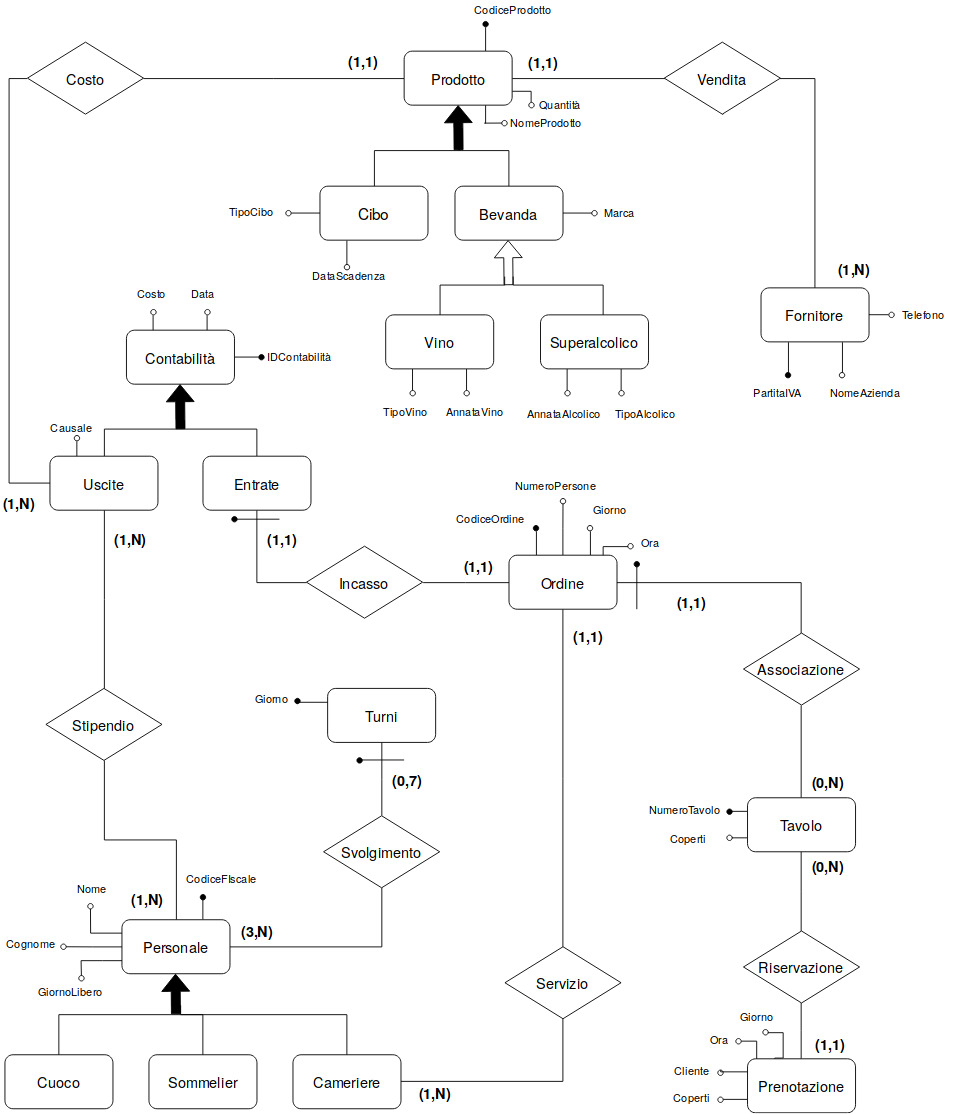
\includegraphics[width=1\textwidth]{doc/schema}
\subsection{Dizionario dei dati}

\textbf{Regole di vincolo} 
\begin{itemize}
    \item Un dipendente non può svolgere più di 6 turni a settimana.
    \item Un cliente non può prenotare un tavolo già prenotato.
    \item Il numero del tavolo deve essere compreso tra 1 e 35.
    \item La quantità del prodotto non può essere negativa.
\end{itemize}

\textbf{Lista delle entità}
\begin{longtable}{p{2.5cm} p{4cm} p{5cm} p{2.5cm}}
    \toprule
    \textbf{Entità} & \textbf{Descrizione} &   \textbf{Attributi} & \textbf{Identificatore}\\ \midrule
    Prodotto & Provvista del magazzino & CodiceProd, NomeProdotto, Quantità & CodiceProd\\ \midrule
    Cibo & Prodotto commestibile & Eredita da Prodotto, TipoCibo, DataScadenza & CodiceProd \\ \midrule
    Bevanda	& Prodotto da bere & Eredita da prodotto, Marca & CodiceProd\\ \midrule
    Vino & Bevanda alcolica a base di uva & Eredita da bevanda, AnnataVino, TipoVino & CodiceProd \\ \midrule
    Superalcolico & Bevanda con grado alcolico elevato & Eredita da Bevanda, TipoAlcolico, AnnataAlcolico & CodiceProd \\ \midrule
    Fornitore & Azienda fornitrice di prodotti & PartitaIva, NomeAzienda, Telefono & PartitaIva \\ \midrule
    Contabilità & Gestione del denaro del locale & CodiceCont, Costo, Data &CodiceCont \\ \midrule
    Entrata & Entrata di denaro del ristorante & Eredita da contabilità & CodiceCont \\ \midrule
    Uscita & Uscita di denaro dal ristorante & Eredita da contabilità, Causale & CodiceCont \\ \midrule
    Ordine & Ordine effettuato per un determinato tavolo & NumeroTavolo, NumeroPersone, Giorno, Ora & NumeroTavolo, Giorno, Ora\\ \midrule
    Prenotazione & Prenotazione per un tavolo del ristorante & NumeroTavolo, Giorno, Ora, NumeroCoperti, Cliente & Numerotavolo, Giorno, Ora \\ \midrule
    Tavolo & Tavolo presente nel locale & NumeroTavolo, Coperti & NumeroTavolo\\ \midrule
    Personale & Insieme dei dipendenti del locale & CodiceFiscale, Nome, Cognome, GiornoLibero & CodiceFiscale\\ \midrule
    Cuoco & Dipendente addetto alla cucina & Eredita da personale & CodiceFiscale\\ \midrule
    Sommelier & Dipendente addetto alla mescita degli alcolici & Eredita da personale & CodiceFiscale\\ \midrule
    Cameriere & Dipendente che serve ai tavoli & Eredita da personale & CodiceFiscale\\ \midrule
    Turno & Turno di lavoro & Giorno & Giorno\\ 
    \bottomrule	
\end{longtable}

\begin{comment}
    \textbf{Lista delle relazioni} %Dalla relazione di La casa del pellegrino
\begin{longtable}{p{2.5cm} p{3cm} p{5.5cm} p{3cm}}
    \midrule
    \textbf{Relazione} & \textbf{Descrizione} & \textbf{Cardinalità} & \textbf{Entità coinvolte} \\ \midrule
    Vendita & Associa il prodotto al suo fornitore & Un prodotto è venduto da un solo fornitore (1,1) \newline Un fornitore vende uno o più prodotti (1,N) & Prodotto, Fornitore \\ \midrule
    Creazione & Associa il prodotto al piatto & Un prodotto crea uno o più piatti (1,N) \newline Un piatto è creato da almeno un prodotto (1,N) & Prodotto, Piatto \\ \midrule
    Costo & Associa il prezzo del prodotto all'uscita di denaro & Un prodotto costituisce una o più uscite (1,N) \newline Un uscita è costituita da uno o più prodotti (1,N) & Prodotto, Uscite \\ \midrule
    Appartenenza & Associa la bevanda all'ordine & Una bevanda può appartenere ad uno o più ordini (0,N) \newline Un ordine contiene almeno una bevanda (1,N) & Bevanda, Ordine \\ \midrule
    Composizione & Associa il piatto all'ordine & Un piatto può comporre uno o più ordini (0,N) \newline Un ordine è composto da almeno un piatto (1,N) & Piatto, Ordine \\ \midrule
    Incasso & Associa l'ordine all'entrata di denaro & Un ordine genera una sola entrata (1,1) \newline Un'entrata è generata da un solo ordine (1,1) & Ordine, Entrate \\ \midrule
    Associazione & Associa l'ordine al tavolo & Un ordine è associato ad un solo tavolo (1,1) \newline Un tavolo può essere associato ad uno o più ordini (0,N) & Ordine, Tavolo \\ \midrule
    Riservazione & Associa il tavolo alla prenotazione & Un tavolo può essere riservato da uno o più clienti (0,N) \newline Una prenotazione riserva un solo tavolo (1,1) & Tavolo, Prenotazione \\ \midrule
    Servizio & Associa l'ordine al cameriere & Un ordine viene servito da un solo cameriere (1,1) \newline Un cameriere serve uno o più ordini (1,N) & Ordine, Cameriere \\ \midrule
    Svolgimento & Associa il dipendente al turno di lavoro & Un dipendente può svolgere un turno (0,7) \newline Un turno è svolto da almeno un dipendente di ciascuna categoria (3,N) & Personale, Turni \\ \midrule
    Stipendio & Associa lo stipendio del dipendente all'uscita di denaro & Un dipendente genera un'uscita mensile (1,N) \newline Un' uscita è costituita da uno o più stipendi (1,N) & Personale, Uscite \\ \bottomrule
\end{longtable}

\end{comment}
\textbf{Lista delle relazioni} %Come nel libro
\begin{longtable}{p{2.5cm} p{5.5cm} p{3.5cm} p{2.5cm}}
    \midrule
    \textbf{Relazione} & \textbf{Descrizione} & \textbf{Cardinalità} & \textbf{Attributi} \\ \midrule
    Vendita & Associa il prodotto al suo fornitore & Prodotto(1,1) \newline Fornitore(1,N) &  \\ \midrule
    Costo & Associa il prezzo del prodotto all'uscita di denaro & Prodotto(1,1) \newline Uscita(1,N) & \\ \midrule
    Incasso & Associa l'ordine all'entrata di denaro & Ordine(1,1) \newline Entrata(1,1) &  \\ \midrule
    Associazione & Associa l'ordine al tavolo & Ordine(1,1) \newline Tavolo(0,N) &  \\ \midrule
    Riservazione & Associa il tavolo alla prenotazione & Tavolo(0,N) \newline Prenotazione(1,1) &  \\ \midrule
    Servizio & Associa l'ordine al cameriere & Ordine(1,1) \newline Cameriere(1,N) & \\ \midrule
    Svolgimento & Associa il dipendente al turno di lavoro & Personale(3,N) \newline Turno(0,7) & \\ \midrule
    Stipendio & Associa lo stipendio del dipendente all'uscita del ristorante & Dipendente(1,N) \newline Uscita(1,N) &  \\ \bottomrule
\end{longtable}

